%\documentclass[tikz]{standalone}

%\begin{document}

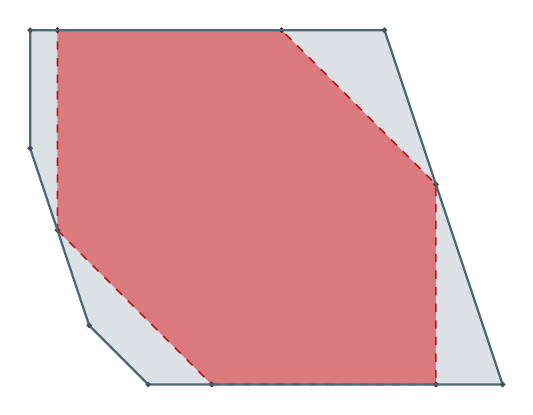
\begin{tikzpicture}%
	[scale=.015,
	edge/.style={color=cyan!40!black, thick},
	facet/.style={fill=cyan!40!black, fill opacity=0.2},
	vertex/.style={inner sep=0pt,circle,draw=cyan!25!black,fill=cyan!75!black,thick,anchor=base},
	edge2/.style={color=red!85!black, dashed, semithick},
	facet2/.style={fill=red, fill opacity=0.500000},
	vertex2/.style={inner sep=0pt,circle,draw=red!40!black,fill=red!75!black,thick,anchor=base}]
%%
%% Drawing the facets
%%
\fill[facet2] (-276.85833996487725, 130.57589164972043) --  (-146.28281540686467, 0.0003670917078508751) --  (43.52500778560571, 0.0003670917078508751) --  (43.52500778560571, 169.4241075639333) -- (-87.0505167724069, 299.9996321219458) --  (-276.85833996487725, 299.9996321219459) -- cycle {};
%%
%% Drawing edges in the front
%%
\draw[edge2] (-276.85833996487725, 130.57589164972043) --  (-146.28281540686467, 0.0003670917078508751) --  (43.52500778560571, 0.0003670917078508751) --  (43.52500778560571, 169.4241075639333) -- (-87.0505167724069, 299.9996321219458) --  (-276.85833996487725, 299.9996321219459) -- cycle {};
%%
%% Drawing the vertices in the front
%%
\node[vertex2] at (-276.85833996487725, 130.57589164972043) {};
\node[vertex2] at (-146.28281540686467, 0.0003670917078508751) {};
\node[vertex2] at (43.52500778560571, 0.0003670917078508751) {};
\node[vertex2] at (43.52500778560571, 169.4241075639333) {};
\node[vertex2] at (-87.0505167724069, 299.9996321219458) {};
\node[vertex2] at (-276.85833996487725, 299.9996321219459) {};
%%
%%
%% Drawing the facets
%%
\fill[facet] (-300.0, 300.0) -- (-300.0, 200.0) -- (-250.0, 50.0) -- (-200.0, 0.0) -- (100.0, 0.0) -- (0.0, 300.0) -- cycle {};
%%
%% Drawing edges in the front
%%
\draw[edge] (-300.0, 300.0) -- (-300.0, 200.0) -- (-250.0, 50.0) -- (-200.0, 0.0) -- (100.0, 0.0) -- (0.0, 300.0) -- cycle {};
%%
%% Drawing the vertices in the front
%%
\node[vertex] at (-300.0, 300.0) {};
\node[vertex] at (-300.0, 200.0) {};
\node[vertex] at (-250.0, 50.0) {};
\node[vertex] at (-200.0, 0.0) {};
\node[vertex] at (100.0, 0.0) {};
\node[vertex] at (0.0, 300.0) {};
%%
\end{tikzpicture}

%\end{document}